% Chapter 4 RKNN-TSVM

\chapter{ماشین بردار پشتیبان دو قلو مبتنی بر رگولارسیون و نزدیک‌ترین همسایه}\label{ch:4}
\section{مقدمه}\label{sec:4:1}
در بخش ‏\ref{sec:2:2:3} برخی از گسترش‌های \lr{TSVM} معرفی شد. بعضی از این گسترش‌ها مبتنی بر رویکرد نزدیک‌ترین همسایه هستند. با وجود اینکه گسترش‌های با رویکرد نزدیک‌ترین همسایه مزیت‌هایی مانند دقت بیشتر را دارند، این روش‌ها سه نقطه ضعف دارند که عبارتند از:
\begin{enumerate}
	\item این روش‌ها به نمونه‌ها بر اساس شمارش تعداد همسایه‌های نزدیک‌شان وزن می‌دهند. بطوریکه فاصله بین نزدیک‌ترین همسایه‌های یک نمونه در نظر گرفته نمی‌شود. نسبت دادن وزن براساس فاصله می‌تواند باعث شناسایی بهتر نواحی پرتراکم شود. به عبارت دیگر، وزن بیشتری به یک نمونه با همسایه‌های نزدیک‌تر داده می‌شود تا به یک نمونه با همسایه‌های دورتر.
	\item این روش‌ها همانند \lr{TSVM} خطای آموزشی (ریسک تجربی) را کمینه می‌کنند. از این رو امکان برازش بیش از حد وجود دارد و تعمیم‌پذیری مدل خروجی کاهش می‌یابد. این نقطه ضعف با در نظر گرفتن ریسک ساختاری در تابع هدف مسئله بهینه‌سازی برطرف می‌شود.
	\item در این روش‌ها، گراف نزدیک‌ترین همسایه با الگوریتم جستجوی کامل\footnote{\lr{Full search algorithm}}  (\lr{FSA}) ساخته می‌شود. مرتبه زمانی این الگوریتم جستجو برابر با  $\mathcal{O}(m^2)$ است. بنابراین اجرای این الگوریتم روی مجموعه داده‌های بزرگ زمان‌بر خواهد بود. اگرچه الگوریتم‌های جدیدی برای ساخت گراف نزدیک‌ترین همسایه ارائه شده است که مرتبه زمانی کمتر از روش \lr{FSA} دارند. در سال 2015، الگوریتم گراف نزدیک‌ترین همسایه مبتنی بر تفاوت مکانی فاصله‌ها (\gls*{LDMDBA}) ارائه شد \cite{xia2015}. مرتبه زمانی روش \lr{LDMDBA} برابر با $\mathcal{O}(\log nm\log m)$ است. این روش جدید می‌تواند به منظور ساخت گراف نزدیک‌ترین همسایه استفاده شود. در نتیجه پیچیدگی محاسباتی کلی دسته بند بهبود می‌یابد.
\end{enumerate} 

در این فصل، با انگیزه‌ی برطرف کردن نقاط ضعف اشاره شده، دسته‌بند ماشین بردار پشتیبان دو قلو مبتنی بر رگولارسیون و نزدیک‌ترین همسایه  (\lr{RKNN-TSVM}) ارائه شده است. روش پیشنهادی برخلاف روش‌های \lr{WLTSVM} و \lr{KNN-LSTSVM}، به نمونه‌های آموزشی بر اساس فاصله بین نزدیک‌ترین همسایه‌هایش وزن می‌دهد. بطوریکه شناسایی نمونه‌های با تراکم بالا و فشردگی درون کلاسی بهبود می‌یابد. همچنین روش \lr{RKNN-TSVM} ریسک ساختاری را کمینه می‌کند. بنابراین مسائل بهینه‌سازی در این روش معین مثبت \footnote{\lr{Positive definite}} هستند.

چالش اصلی روش \lr{RKNN-TSVM}، پیچیدگی محاساباتی بالا برای مجموعه داده‌های بزرگ است. زیرا این روش دو مسئله بهینه‌سازی دوگان حل می‌کند و همچنین \lr{k} نزدیک‌ترین همسایه برای تمام نمونه‌های آموزشی باید محاسبه شود. به منظور بهبود مرتبه زمانی گراف نزدیک‌ترین همسایه، روش‌هایی مانند درخت \lr{k} بعدی (\gls{KDT}) \cite{friedman1977}، درخت \gls{LBT} \cite{chen2007} و روش \lr{LDMDBA} ارائه شده است. روش \lr{LDMDBA} دارای مرتبه زمانی  $\mathcal{O}(\log nm\log m)$ است که از روش \lr{FSA} و بیشتر الگوریتم‌های گراف نزدیک‌ترین همسایه بهتر است. روش \lr{RKNN-TSVM} برای ساخت گراف نزدیک‌ترین همسایه از روش \lr{LDMDBA} استفاده می‌کند.

دسته‌بند ارائه شده در این فصل، یعنی \lr{RKNN-TSVM} دارای مزایای زیر است:  
\begin{itemize}[label=$\bullet$]
	\item	روش \lr{RKNN-TSVM} به نمونه‌ها براساس فاصله نزدیک‌ترین همسایه‌هایش وزن می‌دهد. به عبارت دیگر، نواحی پرتراکم بهتر شناسایی می‌گردد و ابرصفحه به نمونه‌های با تراکم بالا نزدیک‌تر می‌شود. بطوریکه به نمونه‌های با همسایه‌های نزدیک‌تر وزن بیشتری نسبت داده می‌شود.
	\item برخلاف روش \lr{WLTSVM} و \lr{KNN-LSTSVM}، ریسک ساختاری در مسائل بهینه‌سازی روش \lr{RKNN-TSVM} لحاظ شده است. بدین ترتیب دقت و تعمیم‌پذیری مدل خروجی افزایش بهبود می‌یابد.
	\item روش \lr{LDMDBA} جهت بهبود پیچیدگی محاسباتی دسته‌بند بکار گرفته شده است. همچنین این روش برای نسخه غیر خطی دسته‌بند \lr{RKNN-TSVM} نیز موثر می‌باشد. بطوریکه پیدا کردن \lr{k} نزدیک‌ترین همسایه در فضای ویژگی با ابعاد بسیار بالا توسط روش \lr{LDMDBA} بسیار سریعتر از روش \lr{FSA} است.
	\item شیوه وزن‌دهی به یک نمونه در روش \lr{RKNN-TSVM}، براساس فاصله نمونه مورد نظر از نزدیک‌ترین همسایه‌هایش است. بطوریکه مدل خروجی حساسیت کمتری نسبت به نمونه‌های نویزی و پرت دارد.
\end{itemize}

در ادامه این فصل، ابتدا روش \lr{LDMDBA} به طور خلاصه معرفی می‌شود. شیوه جدید وزن دهی در بخش \ref{sec:4:3} بیان شده است. نسخه خطی و غیر خطی دسته‌بند \lr{RKNN-TSVM} به ترتیب در بخش‌های \ref{sec:4:4} و \ref{sec:4:5} شرح داده می‌شود. سپس دسته‌بند\lr{RKNN-TSVM} در بخش \ref{sec:4:6} تحلیل و بررسی می‌شود.

\section{الگوریتم نزدیک‌ترین همسایه مبتنی بر تفاوت مکانی فاصله‌ها}\label{sec:4:2}
الگوریتم \lr{LDMDBA} مفهوم تفاوت مکانی را معرفی کرد \cite{xia2015}. ایده اصلی این است که همسایه‌ها راجع به مکان‌شان اطلاعات مشابه‌ای دارند. به منظور شرح بهتر، شکل \ref{fig:LDMDBA}  ایده روش \lr{LDMDBA} را نشان می‌دهد.

\begin{figure}[!b]
	\centering
	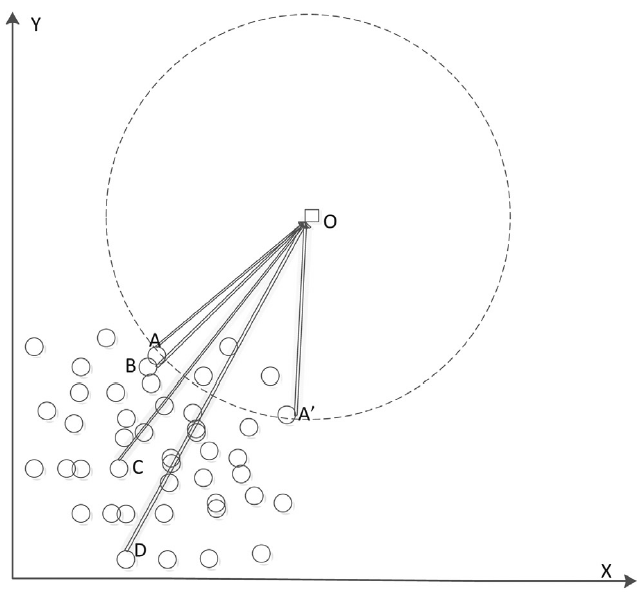
\includegraphics[scale=0.5]{LDMDBA-Idea}
	\caption[ایده اصلی روش \lr{LDMDBA}]{ایده اصلی روش \lr{LDMDBA} \cite{xia2015}}
	\label{fig:LDMDBA}
\end{figure}

همانطور که در شکل  \ref{fig:LDMDBA}‏ نشان داده شده است، تفاوت مکانی همسایه‌ها از طریق فاصله آن‌ها از نقطه مرجع $O$ اندازه‌گیری می‌شود. برای مثال، نمونه  $A$ همسایه نزدیک نمونه $B$  است. زیرا فاصله هر دو نمونه از نقطه مرجع  بسیار مشابه یکدیگر است. با این حال فاصله از یک نقطه مرجع برای پیدا کردن دقیق نزدیک‌ترین همسایه‌ها کافی نمی‌باشد. بنابراین فاصله از چندین نقطه مرجع محاسبه می‌شود.

به منظور بیان الگوریتم \lr{LDMDBA}، مسئله پیدا کردن  $k$نزدیک‌ترین همسایه با مجموعه داده $T=\{(x_1, y_1),\dots,(x_m, y_m)\}$ را در نظر می‌گیریم. فاصله یک نمونه   $x_{j} \in T$ از نقطه مرجع $O_{1}$  به این صورت $Dis_{1}(x_{j})=\left\|x_{j}-O_{1}\right\|$  نشان داده می‌شود. . تعداد نقاط مرجع طبق مقاله اصلی \cite{xia2015} برابر با  ${{\log }_{2}}n$ است ($n$  بیانگر تعداد ویژگی‌ها است.). مقادیر $i$ بعد اول  $i$مین نقطه مرجع $O_{i}$  مساوی با 1- و سایر مقادیر برابر با 1 است. به عبارت دیگر، نقطه مرجع  $i$ام به این صورت   $O_{i}=(-1,-1,\dots,-1,1,\dots,1)$ است. همچنین $Nea_{i}(x_{j})$ نشان‌دهنده همسایه‌های نمونه $x_j$ است که توسط نقطه مرجع $i$ام مشخص شده است.

به منظور بدست آوردن مجموعه  $Nea_{i}(x_{j})$ ، ابتدا فاصله نمونه  $x_j$ از تمام نقاط مرجع محاسبه می‌شود. بعد از مرتب‌سازی فاصله‌ها، یک دنبال مرتب شده بدست می‌آید. بطوریکه $k$نزدیک‌ترین همسایه نمونه $x_j$  در یک زیردنباله با مرکزیت نمونه  $x_j$  قرار دارد. طول زیردنباله برابر با  $2k*\varepsilon$ است. بطوریکه مقدار $\varepsilon$  مساوی با  ${{\log }_{2}}{{\log }_{2}}m$ می‌باشد (نحوه انتخاب مقدار $\varepsilon$  در مقاله اصلی \cite{xia2015} ذکر شده است.).  در آخر، فاصله اقلیدسی تمام نمونه‌ها در زیردنباله محاسبه می‌شود. آن دسته از نمونه‌های متناظر با  $k$کوچک‌ترین فاصله در زیردنباله به عنوان $k$نزدیک‌ترین همسایه نمونه $x_j$ شناخته می‌شوند. در جمع‌بندی این بخش، الگوریتم \lr{LDMDBA} به صورت گام به گام در الگوریتم \ref{algo:LDMDBA} بیان می‌شود.

\begin{algorithm}[!t]
\begin{steps}
	
	ابتدا مجموعه آموزشی $T$ را در نظر می‌گیریم. سپس مقدار $k$ یعنی تعداد نزدیک‌ترین همسایه‌ها مشخص می‌گردد. با در نظرگرفتن $i=1$،  $k$نزدیک‌ترین همسایه با طی کردن گام‌های زیر بدست می‌آید.
	
	\begin{enumerate}
		\item  $i$مین نقطه مرجع  $O_{i}$ به عنوان یک بردار در نظر گرفته می‌شود که   $i$بعد اول آن برابر 1- است. سایر مقادیر این بردار را مقادیر 1 تشکیل می‌دهد.
		\item 	فاصله تمام نمونه‌ها از نقطه مرجع $O_{i}$  با استفاده از $Dis_{i}(x_{j})=\left\|x_{j}-O_{i}\right\|$  محاسبه می‌شود.
		\item 	تمام نمونه‌ها بر اساس مقدار $Dis_{i}$  مرتب می‌شود و یک دنباله مرتب شده بدست می‌آید.
		\item 	یک زیردنباله‌ای از نمونه‌ها با اندازه  $2k*{{\log }_{2}}{{\log }_{2}}m$ و  $x_{j}$ به عنوان نمونه مرکز را در نظر گرفته می‌شود. سپس فاصله اقلیدسی نمونه  $x_{j}$ از تمام نمونه‌های زیردنباله محاسبه می‌گردد.
		\item فاصله‌های محاسبه شده در گام 4 مرتب می‌شود.
		\item  $k$کوچک‌ترین فاصله در زیردنباله مرتب شده،  $k$نزدیک‌ترین همسایه نمونه  $x_{j}$ هستند.
		\item چنانچه همسایه تمام نمونه‌ها با استفاده از همه نقاط مرجع محاسبه گردد، الگوریتم خاتمه می‌یابد. در غیر این صورت،  $i=i+1$ و الگوریتم در گام 1 ادامه می‌یابد.
	\end{enumerate}

\end{steps}
\caption{الگوریتم نزدیک‌ترین همسایه مبتنی بر تفاوت مکانی فاصله‌ها (\lr{LDMDBA})}
\label{algo:LDMDBA}
\end{algorithm}

مرتبه زمانی الگوریتم \lr{LDMDBA} توسط گام‌های 3 و 5 مشخص می‌شود. مرتبه زمانی الگوریتم مرتب‌سازی استفاده شده در این گام‌ها برابر با   $\mathcal{O}(m{{\log }_{2}}m)$ است. بنابراین پیچیدگی محاسباتی کلی الگوریتم \lr{LDMDBA} مساوی با  $\mathcal{O}(\log nm\log m)$ خواهد بود. مرتبه زمانی الگوریتم \lr{FSA} برابر با  $\mathcal{O}({{m}^{2}}{{\log }_{2}}m)$ است که از الگوریتم \lr{LDMDBA } بیشتر است.

مزیت مهم دیگر الگوریتم \lr{LDMDBA} این است که از ساختار درختی استفاده نمی‌کند. درنتیجه این الگوریتم برای داده‌های با ابعاد بسیار بالا موثر است. نتایج ارزیابی در مقاله اصلی \cite{xia2015}، برتری این الگوریتم را نسبت به \lr{FSA} و سایر الگوریتم‌های نزدیک‌ترین همسایه نشان می‌دهد.

\section{تعریف ماتریس وزن‌ها}\label{sec:4:3}
گسترش‌های \lr{TSVM} مبتنی بر رویکرد نزدیک‌ترین همسایه \cite{ye2012,pan2015,xu2016}، گراف $G$ را برای مدل کردن شباهت نمونه‌ها به صورت زیر تعریف می‌کنند.
\begin{equation}\label{eq:4:1}
W_{ij} =
\begin{cases}
1, & \textrm{\lr{if }} x_i \in Nea\left(x_j\right) \textrm{\lr{ or }} x_j \in Nea\left(x_i\right),  \\
0, & \textrm{\lr{otherwise}}.
\end{cases}
\end{equation}

در رابطه \ref{eq:4:1}، مجموعه $Nea\left(x_j\right)$ به صورت زیر تعریف می‌شود.
\begin{equation}\label{eq:4:2}
Nea(x_j) = \{x^{i}_{j} \mid \textrm{\lr{if }} x^{i}_{j} \textrm{\lr{ is a knn of }} x_{j} ,1 \leq i \leq k \}
\end{equation}

مجموعه $Nea\left(x_j\right)$  بر اساس فاصله اقلیدسی $d(x_{j},x^{i}_{j})$ بین نمونه $x_{i}$ و $x_{j}$  مرتب است.
\begin{equation}\label{eq:4:3}
d(x_{j},x^{i}_{j})= \sqrt{(x_{j} - x^{i}_{j})^{T}(x_{j} - x^{i}_{j})}
\end{equation}
با این حال گراف \ref{eq:4:1} یک نقطه ضعف دارد. مقدار $W_{ij}$ برابر 1 یا 0 است. بطوریکه بین هر کدام از نزدیک‌ترین همسایه‌های نمونه $x_j$ تمایزی قائل نمی‌شود. به منظور بهبود شیوه وزن‌دهی، وزن به یک نمونه بر اساس فاصله بین نزدیک‌ترین همسایه‌هایش نسبت داده می‌شود. گراف $G$ در روش \lr{RKNN-TSVM} با گرفتن ایده از \cite{dudani1976,gou2012} به صورت زیر بازتعریف شده است.
\begin{equation}\label{eq:4:4}
W_{ij} =
\begin{cases}
\acute{w_{ij}}, & \textrm{\lr{if }} x_{i} \in Nea\left(x_{j}\right) \textrm{\lr{ or }} x_j \in Nea\left(x_i\right), \\
0, & \textrm{\lr{otherwise}}.
\end{cases}
\end{equation}

در رابطه \ref{eq:4:4}، $\acute{w_{ij}}$  نشان‌دهنده وزن  $i$مین نزدیک‌ترین همسایه نمونه $x_{j}$  که به صورت زیر تعریف می‌شود.
\begin{equation}\label{eq:4:5}
\acute{w_{ij}} =
\begin{cases}
\frac{d(x_{i},x^{k}_{j}) - d(x_{i},x_{j})}{d(x_{i},x^{k}_{j}) - d(x_{i},x^{1}_{j})}, & \textrm{\lr{if }} d\left(x_{i},x^{k}_{j} \right) \neq d\left(x_{i},x^{1}_{j} \right),  \\
1, & \textrm{\lr{if }} d\left(x_{i},x^{k}_{j} \right) = d\left(x_{i},x^{1}_{j} \right).
\end{cases}
\end{equation}

بر اساس رابطه \ref{eq:4:5}، نمونه  $x_{i}$ با فاصله کمتر وزن بیشتری می‌گیرد نسبت به نمونه‌ای با فاصله بیشتر. بنابراین مقادیر $\acute{w_{ij}}$  به صورت خطی بین بازه $\left[0,1\right]$ قرار می‌گیرد.

به منظور مدل کردن اطلاعات درون و برون کلاسی بر اساس فاصله بین نزدیک‌ترین همسایه‌ها، گراف درون کلاسی $G_{s}$ و گراف برون کلاسی $G_{d}$ به ترتیب در روابط \ref{eq:4:6} و \ref{eq:4:7} تعریف شده است.
\begin{equation}\label{eq:4:6}
W_{s,ij} =
\begin{cases}
\acute{w_{ij}}, & \textrm{\lr{if }} x_{i} \in Nea_{s}\left(x_{j}\right) \textrm{\lr{ or }} x_j \in Nea_{s}\left(x_i\right), \\
0, & \textrm{\lr{otherwise}}.
\end{cases}
\end{equation}
\begin{equation}\label{eq:4:7}
W_{d,ij} =
\begin{cases}
\acute{w_{ij}}, & \textrm{\lr{if }} x_{i} \in Nea_{d}\left(x_{j}\right), \\
0, & \textrm{\lr{otherwise}}.
\end{cases}
\end{equation}

مجموعه‌های $Nea_{s}\left(x_{j}\right)$ و $Nea_{d}\left(x_{j}\right)$ به ترتیب نشان‌دهنده  $k$نزدیک‌ترین همسایه نمونه $x_{j}$  در کلاس مثبت و منفی است. این دو مجموعه در رابطه زیر تعریف شده‌اند.
\begin{align}
\label{eq:4:8}
\begin{split}
Nea_{s}\left(x_j\right) = \{x^{i}_{j} \mid l(x^{i}_{j}) = l(x_{j}), 1 \leq i \leq k \}
\end{split}\\
\label{eq:4:9}
\begin{split}
Nea_{d}\left(x_j\right) = \{x^{i}_{j} \mid l(x^{i}_{j}) \neq l(x_{j}), 1 \leq i \leq k \}
\end{split}
\end{align}

در رابطه \ref{eq:4:8} و \ref{eq:4:9}، $l(x_{j})$  نشان‌دهنده برچسب نمونه $x_{j}$ است. بدیهی است که  $Nea_{s}(x_j)\,\cap\, Nea_{d}(x_j)= \varnothing$ و $Nea_{s}(x_j)\, \cup \, Nea_{d}(x_j) = Nea(x_j)$  برقرار است. زمانی‌که  $W_{s,ij} \neq 0$ یا  $W_{d,ij} \neq 0$، یک یال بی‌جهت به گره $x_{i}$ و $x_{j}$  در گراف متناظرش اضافه می‌شود.

برخلاف روش \lr{TSVM}، فقط بردار‌های پشتیبان به جای کل نمونه‌های آموزشی در ایجاد ابرصفحه بهینه کلاس متناظر اهمیت دارند. به منظور استخراج بردار‌های پشتیبان (نمونه‌های حاشیه‌ای) از نمونه‌های کلاس منفی، ماتریس وزن  $W_{d}$ به صورت زیر بازتعریف می‌شود.
\begin{equation}\label{eq:4:10}
f_{j} =
\begin{cases}
1, & \exists j, W_{d,ij} \neq 0,  \\
0, & \textrm{\lr{otherwise}}.
\end{cases}
\end{equation}

\section{نسخه خطی}\label{sec:4:4}
روش پیشنهادی مشابه روش \lr{TSVM} دو ابرصفحه غیر موازی را ایجاد می‌کند. با این حال هر ابرصفحه به نمونه‌های پرتراکم کلاس خودش نزدیک می‌شود. همچنین روش پیشنهادی ریسک ساختاری را کمینه می‌کند. در حالی‌که در روش \lr{TSVM} خطای آموزشی یا ریسک تجربی کمینه می‌شود. شکل  \ref{fig:RKNN-TSVM} ایده اصلی روش \lr{RKNN-TSVM} را روی یک مجموعه داده مصنوعی نشان می‌دهد.
\begin{figure}[!b]
	\centering
	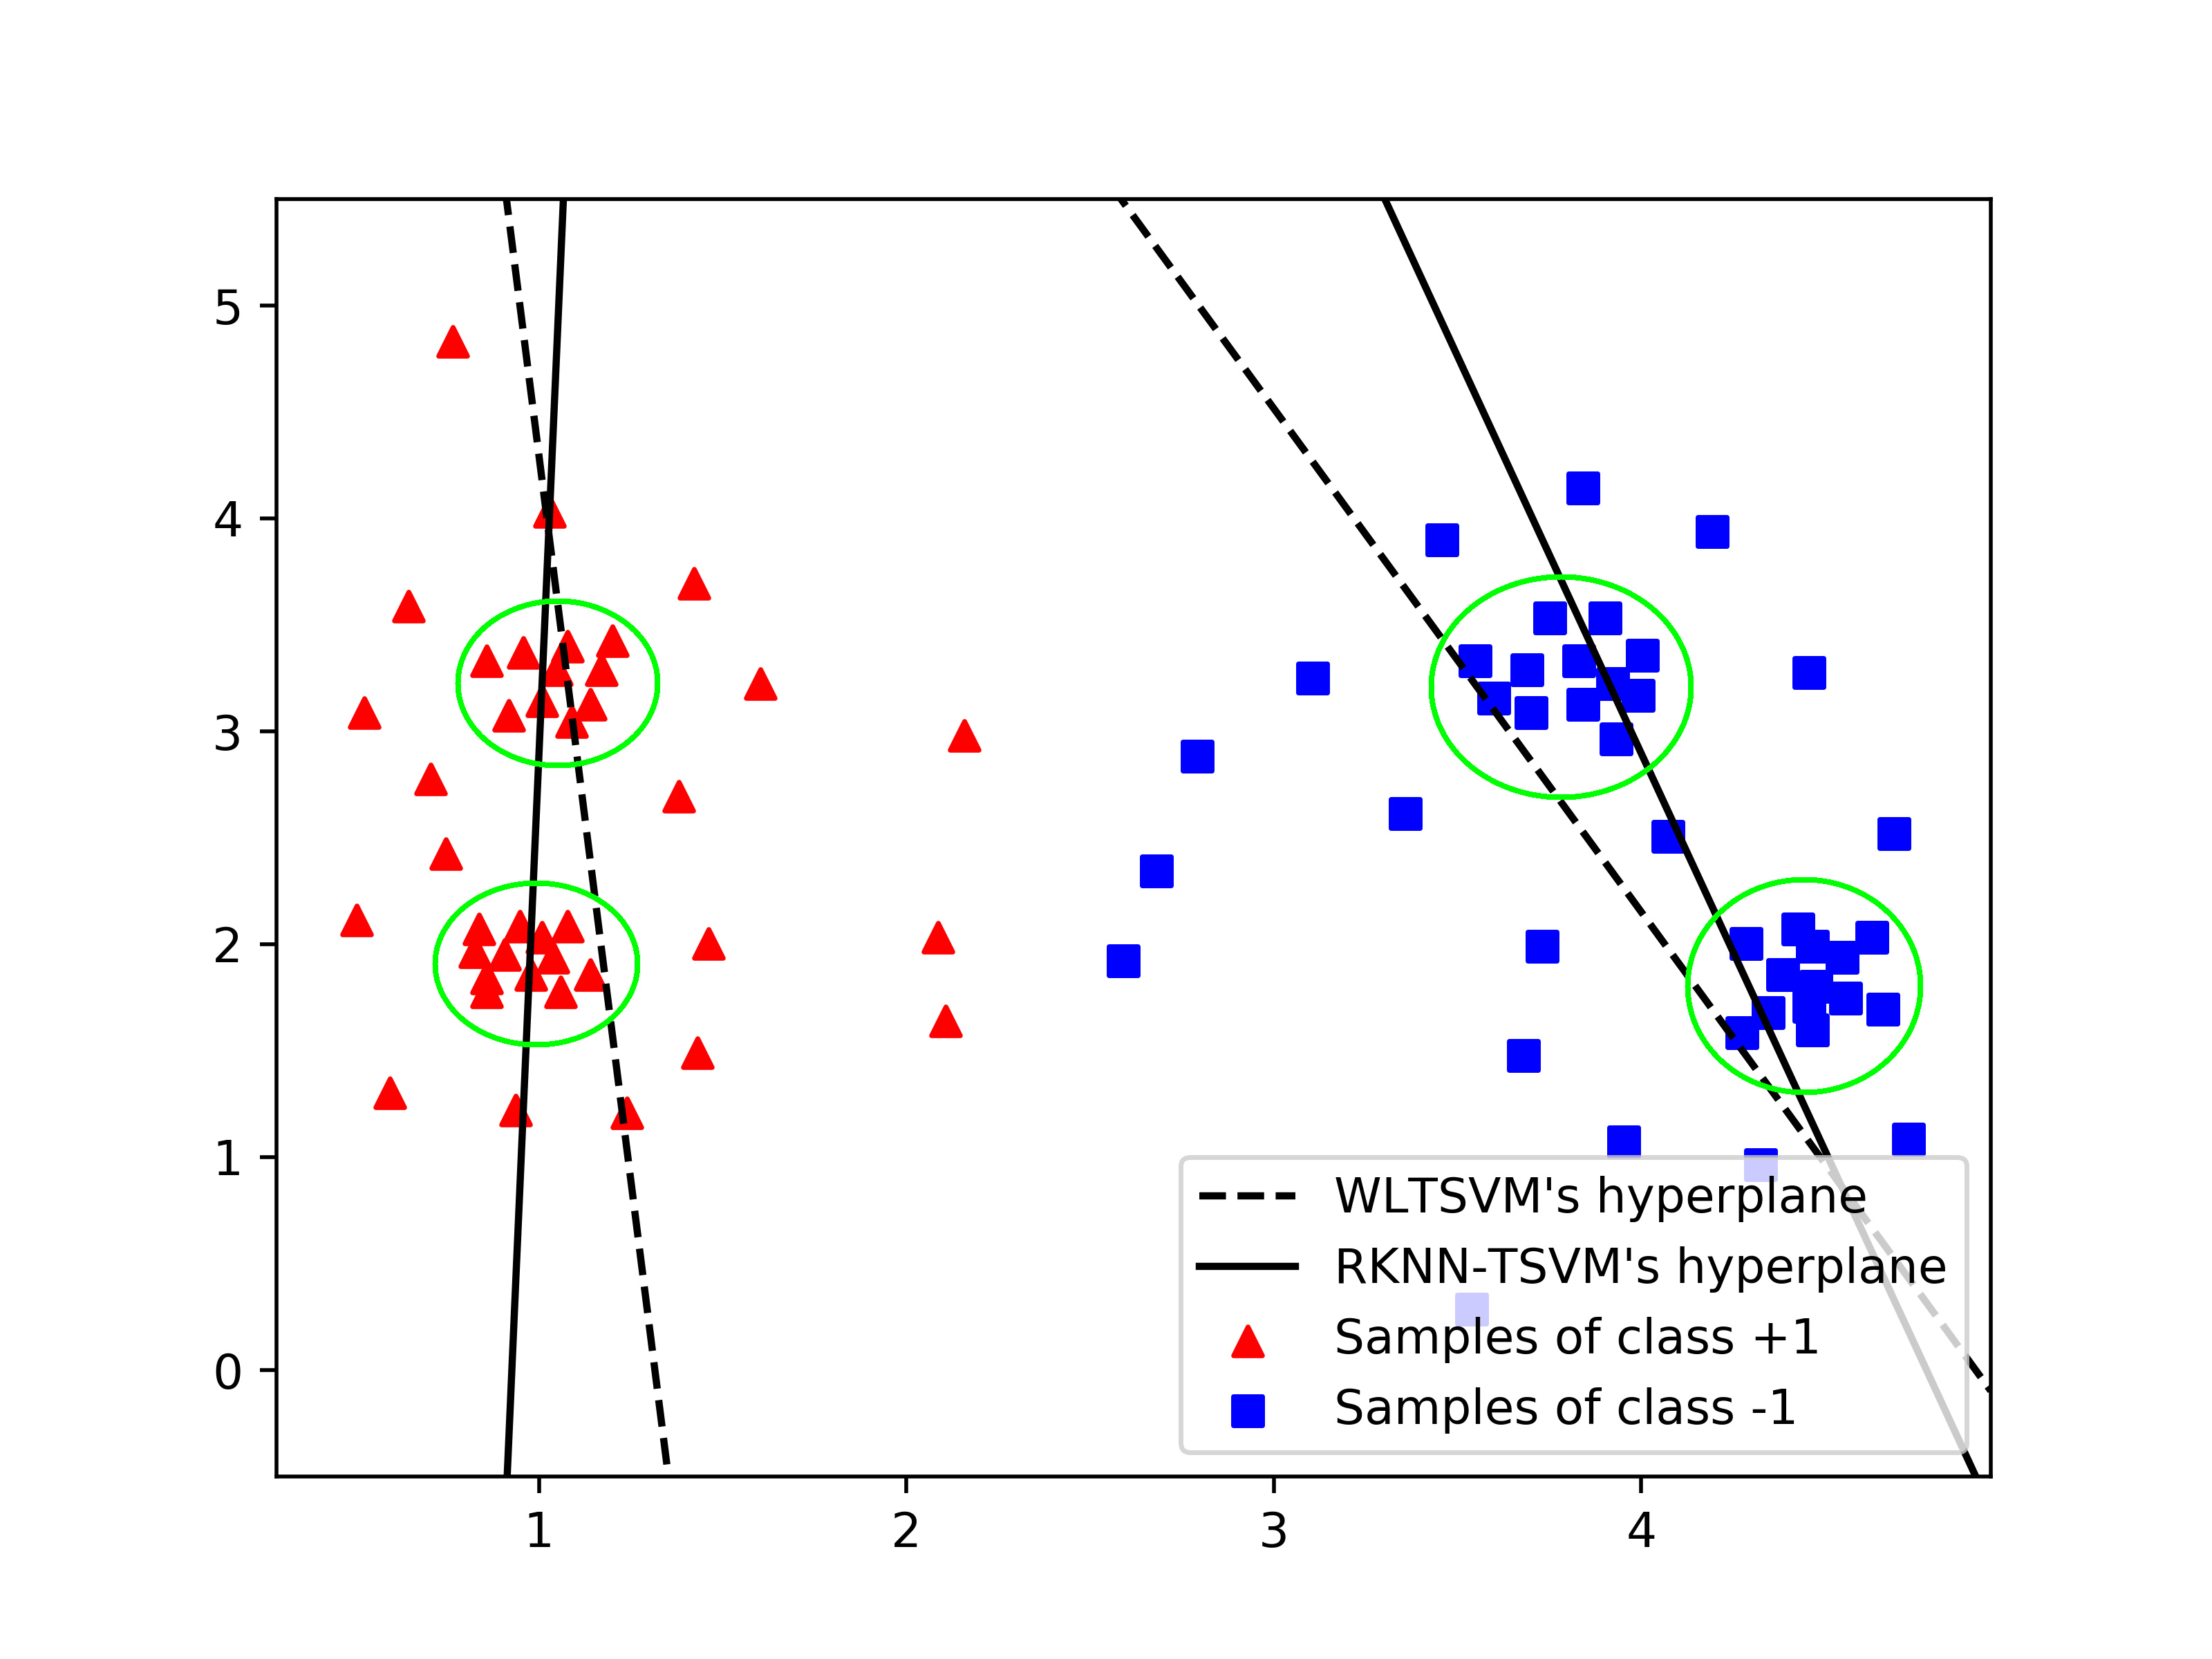
\includegraphics[scale=0.6]{RKNN-TSVM-idea}
	\caption{ ایده اصلی روش \lr{RKNN-TSVM}}
	\label{fig:RKNN-TSVM}
\end{figure}

در شکل ‏\ref{fig:RKNN-TSVM}، دایره‌های سبز رنگ نواحی پرتراکم را نشان می‌دهد. ابرصفحه روش \lr{RKNN-TSVM} نسبت به روش \lr{WLTSVM} به نواحی پرتراکم نزدیک‌تر است. زیرا روش \lr{RKNN-TSVM} به نمونه‌ها براساس فاصله‌شان از نزدیک‌ترین همسایه‌ها وزن می‌دهد. بطوریکه روش پیشنهادی حساسیت کمتری نسبت به نمونه‌های پرت و نویزی دارد.

بعد از محاسبه ماتریس وزن کلاس مثبت  $W^{(1)}_{s_ij}$ و نمونه‌های حاشیه‌ای کلاس منفی  $f^{(2)}_{j}$، مسائل بهینه‌سازی اصلی روش پیشنهادی با در نظر گرفتن ریسک ساختاری به صورت زیر تعریف می‌شوند.
\begin{equation}
\label{eq:4:11}
\begin{split}
\mathop{{ min}}\limits_{w_{1} ,b_{1}} \quad & \frac{1}{2}\sum\limits_{i=1}^{m_{1}}{d^{(1)}_{j}(w^{T}_{1}x^{(1)}_{j}+b_{1})^{2}}+c_{1}e_{2}^{T}\xi+\frac{c_{2}}{2}(\left\|w_{1}\right\|^{2}+b^{2}_{1}) \\
\textrm{\lr{s.t. }} \quad & -f^{(2)}_{j}(w^{T}_{1}x^{(2)}_{j}+b_{1})+\xi_{j} \ge f^{(2)}_{j} \\
& \xi_{j} \ge 0,\quad j=1,...,m_{2}
\end{split}
\end{equation}
\begin{equation}
\label{eq:4:12}
\begin{split}
\mathop{{ min}}\limits_{w_{2} ,b_{2}} \quad & \frac{1}{2}\sum\limits_{i=1}^{m_{2}}{d^{(2)}_{j}(w^{T}_{2}x^{(2)}_{j}+b_{2})^{2}}+c_{1}e_{1}^{T}\eta+\frac{c_{3}}{2}(\left\|w_{2}\right\|^{2}+b^{2}_{2}) \\
\textrm{\lr{s.t. }} \quad & f^{(1)}_{j}(w^{T}_{2}x^{(1)}_{j}+b_{2})+\eta_{j} \ge f^{(1)}_{j} \\
& \eta_{j} \ge 0,\quad j=1,...,m_{1}
\end{split}
\end{equation}

در روابط \ref{eq:4:11} و  \ref{eq:4:12}،  $c_{1},c_{2},c_{3} \geq 0$ پارامترهای مثبت، $\xi $ و  $\eta$ متغیر لغزش مثبت،    $e_{1}$ و  $e_{2}$ به ترتیب بردار ستونی با ابعاد  $m_{1}$ و $m_{2}$  هستند. همچنین  $d^{(1)}_{j}$ نشان‌دهنده وزن نمونه   $x^{(1)}_{j}$ که در رابطه زیر تعریف شده است.
\begin{equation}\label{eq:4:13}
d^{(1)}_{j}=\sum^{n_1}_{i=1} W^{(1)}_{s,ij},j=1,2,\dots,n_1
\end{equation}

تفاوت بین مسائل بهینه‌سازی اصلی روش پیشنهادی و گسترش‌های روش \lr{TSVM} مبتنی بر گراف نزدیک‌ترین همسایه عبارتند از:

\begin{enumerate}
	\item برخلاف روش \lr{WLTSVM}، مقدار   به$d^{(1)}_{j}$ فاصله میان  $k$نزدیک‌ترین همسایه نمونه  $x^{(1)}_{j}$ بستگی دارد. به عبارت دیگر، مقدار  $d^{(1)}_{j}$ نشان دهنده تراکم نمونه $x^{(1)}_{j}$  است.
	\item در مسائل بهینه‌سازی اصلی  \ref{eq:4:11} و \ref{eq:4:12}، ریسک ساختاری با اضافه شدن جمله رگولارسیون   $\frac{c_{2}}{2}(\left\|w_{1}\right\|^{2}+b^{2}_{1})$ کمینه می‌شود. در حالی که خطای نمونه آموزشی در گسترش‌های روش \lr{TSVM} مبتنی بر گراف نزدیک‌ترین همسایه کمینه می‌گردد.
\end{enumerate}

همچنین روش پیشنهادی (\lr{RKNN-TSVM}) مزیت‌های گسترش‌های مبتنی بر گراف نزدیک‌ترین همسایه را دارد که عبارتند از:
\begin{enumerate}
	\item مسائل بهینه‌سازی \ref{eq:4:11} و \ref{eq:4:12} \gls{Convex} و از نوع برنامه‌ریزی درجه دو هستند. بطوریکه این مسائل راه حل بهینه سراسری دارند.
	\item همانند روش \lr{WLTSVM}، پیچیدگی زمانی روش پیشنهادی با در نظر گرفتن نمونه‌های حاشیه‌ای در قید مسئله بهینه‌سازی بهبود یافته است.
\end{enumerate}

به منظور حل کردن مسئله بهینه‌سازی \ref{eq:4:11}، تابع لاگرانژ به صورت زیر تعریف شده است.
\begin{equation}
\begin{split}
L_{1}(w_{1},b_{1},\xi, \alpha, \gamma)= &\frac{1}{2}\sum\limits_{i=1}^{m_{1}}{d^{(1)}_{j}(w^{T}_{1}x^{(1)}_{j}+b_{1})^{2}}+c_{1}e_{2}^{T}\xi+\frac{c_{2}}{2}(\left\|w_{1}\right\|^{2}+b^{2}_{1}) \\
& -\sum\limits_{i=1}^{m_{2}}{\alpha_{j}(-f^{(2)}_{j}(w^{T}_{1}x^{(2)}_{j}+b_{1})+\xi_{j} - f^{(2)}_{j})} - \gamma^{T}\xi
\end{split}
\label{eq:4:14}
\end{equation}

در رابطه \ref{eq:4:14}،  $\alpha=(\alpha_{1}, \alpha_{2}, \dots,\alpha_{n_{2}})^{T}$ و $\gamma=(\gamma_{1}, \gamma_{2}, \dots, \gamma_{n_{2}})^{T}$ بردارهای ضرایب لاگرانژ هستند. با مشتق‌گیری از تابع \ref{eq:4:14} نسبت به   $w_{1}$،  $b_{1}$ و  $\xi$، شرایط \lr{KKT} زیر برقرار می‌شود.
\begin{align}
\label{eq:4:15}
\begin{split}
\frac{\partial L_{1}}{\partial w_{1}}&= \sum\limits_{i=1}^{m_{1}}{d^{(1)}_{j}x^{(1)}_{j}(w^{T}_{1}x^{(1)}_{j} + b_{1})} + c_{2}w_{1} + \sum\limits_{i=1}^{m_{2}}{\alpha_{j}f_{j}^{(2)}x_{j}^{(2)}}=0,
\end{split} \\
\label{eq:4:16}
\begin{split}
\frac{\partial L_{1}}{\partial b_{1}}&= \sum\limits_{i=1}^{m_{1}}{d^{(1)}_{j}(w^{T}_{1}x^{(1)}_{j} + b_{1})} + c_{2}b_{1} +\sum\limits_{i=1}^{m_{2}}{\alpha_{j}f_{j}^{(2)}}=0,
\end{split}\\
\label{eq:4:17}
\begin{split}
\frac{\partial L_{1}}{\partial \xi}&= c_{1}e_{2} - \alpha - \gamma =0,
\end{split}\\
\label{eq:4:18}
\begin{split}
\alpha \geq 0,\, \gamma \geq 0.
\end{split}
\end{align}

با قرار دادن روابط \ref{eq:4:15} و \ref{eq:16}  به صورت فرم ماتریسی، معادلات زیر بدست می‌آید.
\begin{align}
\label{eq:4:19}
\begin{split}
A^{T}D(Aw_{1}+e_{1}b_{1})+c_{2}w_{1}+B^{T}F\alpha=0,
\end{split} \\
\label{eq:4:20}
\begin{split}
e^{T}_{1}D(Aw_{1}+e_{1}b_{1}) + c_{2}b_{1}+e^{T}_{2}F\alpha=0,
\end{split}
\end{align}

در روابط \ref{eq:4:19} و \ref{eq:4:20}،  $D=diag(d^{(1)}_{1},d^{(1)}_{2},\dots,d^{(1)}_{m_{1}})$ و  $F=diag(f^{(2)}_{1},f^{(2)}_{2},\dots,f^{(2)}_{m_{2}})$ ماتریس‌های قطری هستند. در اینجا $d^{(1)}_{j} \geq 0$ و  $f^{(2)}_{j}$ مقدار برابر با 0 یا 1 است. با توجه به اینکه  $\gamma \geq 0$، از رابطه \ref{eq:4:17} خواهیم داشت:
\begin{equation} \label{eq:4:21}
0e_{2} \leq \alpha \leq c_{1}e_{2}
\end{equation}

با ترکیب کردن روابط \ref{eq:4:19} و \ref{eq:4:20} معادله زیر بدست می‌آید.
\begin{equation}\label{eq:4:22}
([A^{T}\ e^{T}_{1}]D[A\ e_{1}] + c_{2}I)[w_{1}\ b_{1}]^{T} + [B^{T}\ e^{T}_{2}]F\alpha = 0.
\end{equation}

در رابطه \ref{eq:4:22}، $I$  ماتریس همانی با ابعاد مناسب است. با تعریف کردن ماتریس‌های $H=[A\,e_{1}]$ و  $G=[B\,e_{2}]$، رابطه \ref{eq:4:22} به صورت زیر بازنویسی می‌شود.
\begin{align}\label{eq:4:23}
\begin{aligned}
&(H^{T}DH+c_{2}I)\left[ \begin{matrix}
{{w}_{1}}  \\
{{b}_{1}}  \\
\end{matrix} \right] + G^{T}F\alpha=0. \\
&i.e., \left[ \begin{matrix}
{{w}_{1}}  \\
{{b}_{1}}  \\
\end{matrix} \right] = -(H^{T}DH+c_{2}I)^{-1}G^{T}F\alpha
\end{aligned}
\end{align}

با توجه به رابطه \ref{eq:4:14} و شرایط \lr{KKT} ذکر شده، حالت دوگان مسئله \ref{eq:4:11} در رابطه زیر تعریف شده است.
\begin{equation}\label{eq:4:24}
\begin{split}
\mathop{{max}}\limits_{\alpha} \quad & e_{2}^{T}F\alpha-\frac{1}{2}{{\alpha }^{T}}(F^{T}G){(H^{T}DH+c_{2}I)^{-1}}{({G}^{T}F)}\alpha   \\
\textrm{\lr{s.t. }} \quad & 0{{e}_{2}}\le \alpha \le {c_{1}}{{e}_{2}}
\end{split}
\end{equation}

لازم به ذکر است که پارامتر $c_{2}$ در مسئله دوگان \ref{eq:4:24} می‌تواند با $\varepsilon > 0$ جایگزین شود. بطوریکه پارامتر  $\varepsilon$ یک عدد ثابت بسیار کوچک مانند $\varepsilon=1e-8$ است. در حالی‌که پارامتر  $c_{2}$ تعادل بین جمله رگولارسیون و ریسک تجربی را تعیین می‌کند \cite{shao2011}.

مشابه کلاس مثبت، تابع لاگرانژ مسئله اصلی کلاس منفی \ref{eq:4:12} به صورت زیر تعریف می‌شود.
\begin{align}\label{eq:4:25}
\begin{aligned}
L_{2}(w_{2},b_{2},\eta, \beta, \nu)= &\frac{1}{2}\sum\limits_{i=1}^{n_{2}}{d^{(2)}_{j}(w^{T}_{2}x^{(2)}_{j}+b_{2})^{2}}+c_{1}e_{1}^{T}\eta+\frac{c_{3}}{2}(\left\|w_{2}\right\|^{2}+b^{2}_{2}) \\
& -\sum\limits_{i=1}^{n_{1}}{\beta_{j}(f^{(1)}_{j}(w^{T}_{2}x^{(2)}_{j}+b_{2})+\eta_{j} - f^{(1)}_{j})} - \nu^{T}\eta
\end{aligned}
\end{align}

در رابطه \ref{eq:4:25}،  $\beta=(\beta_{1}, \beta_{2}, \dots,\beta_{n_{1}})^{T}$ و $\nu=(\nu_{1}, \nu_{2}, \dots,\nu_{n_{1}})^{T}$ بردارهای ضرایب لاگرانژ هستند. با مشتق‌گیری از تابع لاگرانژ \ref{eq:4:25} نسبت به  $w_{2}$،  $b_{2}$، و  $\eta$، حالت دوگان مسئله اصلی \ref{eq:4:12} به صورت زیر تعریف می‌شود.
\begin{equation}\label{eq:4:26}
\begin{split}
\mathop{{max}}\limits_{\beta} \quad & e_{1}^{T}P\beta-\frac{1}{2}{{\beta}^{T}}(P^{T}H){(G^{T}QG+c_{3}I)^{-1}}{({H}^{T}P)}\beta   \\
\textrm{\lr{s.t. }} \quad & 0{{e}_{1}}\le \beta \le {c_{1}}{{e}_{1}}
\end{split}
\end{equation}

در رابطه \ref{eq:4:26}،  $Q=diag(d^{(2)}_{1},d^{(2)}_{2},\dots,d^{(2)}_{n_{2}})$ و  $P=diag(f^{(1)}_{1},f^{(1)}_{2},\dots,f^{(1)}_{n_{1}})$ به ترتیب ماتریس وزن کلاس منفی و نمونه‌های حاشیه‌ای کلاس مثبت هستند. همچنین مقدار  $f^{(1)}_{j}$ برابر با 0 یا 1 است. بررسی مسئله دوگان \ref{eq:4:24} و \ref{eq:4:26} نشان می‌دهد که پیچیدگی محاسباتی روش \lr{RKNN-TSVM} وابسته به نمونه‌های حاشیه‌ای است.

زمانی‌که مسئله دوگان \ref{eq:4:26} حل شود، ابرصفحه کلاس منفی از طریق معادله زیر بدست می‌آید.
\begin{equation} \label{eq:4:27}
\left[ \begin{matrix}
{{w}_{2}}  \\
{{b}_{2}}  \\
\end{matrix} \right] = (G^{T}QG+c_{3}I)^{-1}H^{T}P\beta
\end{equation}

کلاس نمونه جدید $x \in \mathbb{R}^{d}$ از طریق تابع تصمیم زیر مشخص می‌شود.
\begin{equation}\label{eq:4:28}
d(x) =
\begin{cases}
+1, & \textrm{\lr{if }} \frac{\left| {{x}^{T}}{{w}_{1}}+{{b}_{1}} \right|}{\left\|w_1\right\|} < \frac{\left| {{x}^{T}}{{w}_{2}}+{{b}_{2}} \right|}{\left\|w_2\right\|} \\
-1, & \textrm{\lr{otherwise}}.
\end{cases}
\end{equation}
مراحل ایجاد مدل خطی دسته‌بند \lr{RKNN-TSVM} در الگوریتم \ref{algo:Linear-RKNN-TSVM} ذکر شده است.
 
\begin{algorithm}[!h]
\begin{steps}

	ابتدا فرض می‌گیریم که مجموعه آموزشی $T=\{(x_1, y_1),\dots,(x_m, y_m)\}$  را در اختیار داریم و $k$ پارامتر یعنی تعداد نزدیک‌ترین همسایه‌ها مشخص شده است. سپس مدل خطی روش \lr{RKNN-TSVM} با طی کردن گام‌های زیر بدست می‌آید.
	
	\begin{enumerate}
		\item به منظور بدست آوردن مجموعه $Nea(x_{j})$ ،  $k$نزدیک‌ترین همسایه هر نمونه  $x_{j} \in T$ را با استفاده الگوریتم \lr{FSA} یا \lr{LDMDBA} پیدا کنید.
		\item ماتریس وزن $W_s$  و $W_d$  برای کلاس مثبت و منفی با استفاده از روابط \ref{eq:4:6} و \ref{eq:4:7}  تعریف می‌شود.
		\item ماتریس‌های قطری  $D$،  $Q$، $F$  و $P$  با استفاده از روابط \ref{eq:4:10} و \ref{eq:4:13} بدست می‌آید.
		\item ابتدا ماتریس‌های ورودی  $A \in \mathbb{R}^{m_1 \times n}$ و   $B \in \mathbb{R}^{m_2 \times n}$معین می‌شود. سپس ماتریس‌های  $H$  و $G$  به این صورت  $H=[A\,e_{1}]$ و $G=[B\,e_{2}]$ تعریف می‌گردد.
		\item پارامترهای  $c_{1}$، $c_{2}$  و $c_{3}$ تعیین می‌شود. این پارامتر معمولا براساس مجموعه داده صحت مشخص می‌شود.
		\item راه حل بهینه $\alpha$  و $\beta$  به ترتیب با حل کردن مسائل \ref{eq:4:24} و \ref{eq:4:26} دوگان بدست می‌آید.
		\item مختصات دو ابرصفحه غیر موازی با حل کردن معادلات \ref{eq:4:23} و \ref{eq:4:27} تعیین می‌شود.
		\item کلاس نمونه جدید  $x \in \mathbb{R}^{n}$ از طریق تابع تصمیم \ref{eq:4:28} مشخص می‌شود.
	\end{enumerate}
\end{steps}
\caption{ایجاد مدل خطی دسته‌بند \lr{RKNN-TSVM}}
\label{algo:Linear-RKNN-TSVM}
\end{algorithm}

در جمع‌بندی نسخه خطی، ذکر دو نکته زیر ضروری است.
\begin{enumerate}
	\item راه حل‌های نسخه خطی \ref{eq:4:23} و \ref{eq:4:27} به ترتیب شامل دو معکوس ماتریس   $(H^{T}DH+c_{2}I)^{-1}$ و  $(G^{T}QG+c_{3}I)^{-1}$ با ابعاد $(n+1)\times(n+1)$  می‌باشد. بطوریکه $n$ بسیار کوچکتر از نمونه‌های آموزشی است ($n \ll m$).
	\item به دلیل اضافه شدن جمله رگولارسیون به تابع هدف، ماتریس‌های   $(H^{T}DH+c_{2}I)$ و   $(G^{T}QG+c_{3}I)$ معین مثبت هستند. بنابراین روش پیشنهادی پایدار است و از شرایط منفرد ماتریس‌های $H^{T}DH$ و $G^{T}QG$  جلوگیری می‌کند.
\end{enumerate}

\section{نسخه غیر خطی}\label{sec:4:5}
در دنیای واقعی، بسیاری از مسائل دسته‌بندی با تابع هسته خطی جدا پذیر نیستند. به منظور جدا سازی مسائل غیر خطی، نمونه‌ها به فضای ویژگی با ابعاد بیشتر نگاشت می‌شوند. بنابراین روش \lr{RKNN-TSVM} با در نظرگرفتن دو ابرسطح زیر به نسخه غیر خطی گسترش می‌یابد.
\begin{equation}\label{eq:4:29}
K(x){{\mu}_{1}}+{{b}_{1}}=0, \quad \textrm{\lr{and}} \quad K(x){{\mu}_{2}}+{{b}_{2}}=0
\end{equation}

در رابطه \ref{eq:4:29}، $K(x)$  نشان دهنده تابع هسته دلخواه است که به صورت زیر تعریف می‌شود.
\begin{equation}\label{eq:4:30}
K(x) = [K(x_{1},x),K(x_{2},x),\dots,K(x_{n},x)]^{T}
\end{equation}

مسائل بهینه‌سازی اصلی نسخه غیر خطی روش \lr{RKNN-TSVM} به صورت زیر تعریف می‌گردد.

\begin{equation}
\label{eq:4:31}
\begin{split}
\mathop{{ min}}\limits_{\mu_{1} ,b_{1}} \quad & \frac{1}{2}\sum\limits_{i=1}^{m_{1}}{d^{(1)}_{j}(\mu^{T}_{1}K(x^{(1)}_{j})+b_{1})^{2}}+c_{1}e_{2}^{T}\xi+\frac{c_{2}}{2}(\left\|\mu_{1}\right\|^{2}+b^{2}_{1}) \\
\textrm{\lr{s.t. }} \quad & -f^{(2)}_{j}(\mu^{T}_{1}K(x^{(2)}_{j}) + b_{1})+\xi_{j} \ge f^{(2)}_{j} \\
& \xi_{j} \ge 0,\quad j=1,...,m_{2}
\end{split}
\end{equation}
\begin{equation}
\label{eq:4:32}
\begin{split}
\mathop{{ min}}\limits_{\mu_{2} ,b_{2}} \quad & \frac{1}{2}\sum\limits_{i=1}^{m_{2}}{d^{(2)}_{j}(\mu^{T}_{2}K(x^{(2)}_{j})+b_{2})^{2}}+c_{1}e_{1}^{T}\eta+\frac{c_{3}}{2}(\left\|\mu_{2}\right\|^{2}+b^{2}_{2}) \\
\textrm{\lr{s.t. }} \quad & f^{(1)}_{j}(\mu^{T}_{2}K(x^{(1)}_{j})+b_{2})+\eta_{j} \ge f^{(1)}_{j} \\
& \eta_{j} \ge 0,\quad j=1,...,m_{1}
\end{split}
\end{equation}

در روابط \ref{eq:4:31} و \ref{eq:4:32}،  $c_{1},c_{2},c_{3}$ پارامترهای مثبت،  $\xi$ و  $\eta$ متغیر لغزش هستند. همچنین   $d_{j}$ و  $f_{j}$ همانند نسخه خطی تعریف می‌شوند. فاصله اقلیدسی نیز در فضای ویژگی با ابعاد بالا محاسبه می‌شود. مشابه نسخه خطی، تابع لاگرانژ مسئله بهینه‌سازی اصلی \ref{eq:4:32} به صورت زیر تعریف می‌شود.

\begin{align}\label{eq:4:33}
\begin{aligned}
L_{1}(\mu_{1},b_{1},\xi, \alpha, \gamma)= &\frac{1}{2}\sum\limits_{i=1}^{n_{1}}{d^{(1)}_{j}(\mu^{T}_{1}K(x^{(1)}_{j})+b_{1})^{2}}+c_{1}e_{2}^{T}\xi+\frac{c_{2}}{2}(\left\|\mu_{1}\right\|^{2}+b^{2}_{1}) \\
& -\sum\limits_{i=1}^{n_{2}}{\alpha_{j}(-f^{(2)}_{j}(\mu^{T}_{1}K(x^{(2)}_{j})+b_{1})+\xi_{j} - f^{(2)}_{j})} - \gamma^{T}\xi
\end{aligned}
\end{align}

در رابطه \ref{eq:4:33}،  $\alpha=(\alpha_{1}, \alpha_{2}, \dots,\alpha_{n_{2}})^{T}$ و  $\gamma=(\gamma_{1}, \gamma_{2}, \dots, \gamma_{n_{2}})^{T}$ نشان دهنده بردارهای ضرایب لاگرانژ هستند. شرایط \lr{KKT} برای  $\mu_{1}$،  $b_{1}$،  $\xi$ و $\alpha$، $\gamma$  به صورت زیر تعریف شده است.
\begin{align}
\label{eq:4:34}
\begin{split}
\frac{\partial L_{1}}{\partial \mu_{1}}&= \sum\limits_{i=1}^{m_{1}}{d^{(1)}_{j}K(x^{(1)}_{j})(\mu^{T}_{1}K(x^{(1)}_{j}) + b_{1})} + c_{2}\mu_{1} + \sum\limits_{i=1}^{m_{2}}{\alpha_{j}f_{j}^{(2)}K(x_{j}^{(2)})}=0,
\end{split} \\
\label{eq:4:35}
\begin{split}
\frac{\partial L_{1}}{\partial b_{1}}&= \sum\limits_{i=1}^{m_{1}}{d^{(1)}_{j}(w^{T}_{1}x^{(1)}_{j} + b_{1})} + c_{2}b_{1} +\sum\limits_{i=1}^{m_{2}}{\alpha_{j}f_{j}^{(2)}}=0,
\end{split}\\
\label{eq:4:36}
\begin{split}
\frac{\partial L_{1}}{\partial \xi}&= c_{1}e_{2} - \alpha - \gamma =0,
\end{split}\\
\label{eq:4:37}
\begin{split}
\alpha \geq 0,\, \gamma \geq 0.
\end{split}
\end{align}

با قرار دادن روابط \ref{eq:4:34} و \ref{eq:4:35} به صورت فرم ماتریسی، معادلات زیر بدست می‌آید.
\begin{align}
\label{eq:4:38}
\begin{split}
K(A)^{T}D(K(A)\mu_{1}+e_{1}b_{1})+c_{2}\mu_{1}+K(B)^{T}F\alpha=0,
\end{split} \\
\label{eq:4:39}
\begin{split}
e^{T}_{1}D(K(A)\mu_{1}+e_{1}b_{1}) + c_{2}b_{1}+e^{T}_{2}F\alpha=0,
\end{split}
\end{align}

در روابط \ref{eq:4:38} و \ref{eq:4:39}، $K(A)$ و $K(B)$ به ترتیب ماتریس‌های هسته با ابعاد  $m_{1} \times m$ و $m_{2} \times m$ هستند ($m=m_{1}+m_{2}$). با توجه به اینکه  $\gamma \geq 0$، از رابطه \ref{eq:37} خواهیم داشت:
\begin{equation}\label{eq:4:40}
0e_{2} \leq \alpha \leq c_{1}e_{2}
\end{equation}

به طرز مشابه‌ای، با ترکیب روابط \ref{eq:4:38} و \ref{eq:4:39} معادله زیر بدست می‌آید.
\begin{equation}\label{eq:4:41}
([K(A)^{T}\ e^{T}_{1}]D[K(A)\ e_{1}] + c_{2}I)[\mu_{1}\ b_{1}]^{T} + [K(B)^{T}\ e^{T}_{2}]F\alpha = 0.
\end{equation}

با تعریف ماتریس‌های  $R=[K(A)\,e_{1}]$ و $S=[K(B)\,e_{2}]$ ، رابطه \ref{eq:4:41} به صورت زیر بازنویسی می‌شود.
\begin{equation}\label{eq:4:42}
\left[ \begin{matrix}
{{\mu}_{1}}  \\
{{b}_{1}}  \\
\end{matrix} \right] = -(R^{T}DR+c_{2}I)^{-1}S^{T}F\alpha
\end{equation}

سپس حالت دوگان مسئله اصلی \ref{eq:4:31} به صورت زیر تعریف می‌گردد.
\begin{equation}\label{eq:4:43}
\begin{split}
\mathop{{max}}\limits_{\alpha} \quad & e_{2}^{T}F\alpha-\frac{1}{2}{{\alpha }^{T}}(F^{T}S){(R^{T}DR+c_{2}I)^{-1}}{({S}^{T}F)}\alpha   \\
\textrm{\lr{s.t. }} \quad & 0{{e}_{2}}\le \alpha \le {c_{1}}{{e}_{2}}
\end{split}
\end{equation}

با جا‌به‌جا کردن نقش‌های  $K(A)$ و $K(B)$  در رابطه \ref{eq:4:43}، حالت دوگان مسئله اصلی \ref{eq:4:32} به صورت زیر بدست
می‌آید.
\begin{equation}\label{eq:4:44}
\begin{split}
\mathop{{max}}\limits_{\beta} \quad & e_{1}^{T}P\beta-\frac{1}{2}{{\beta}^{T}}(P^{T}R){(S^{T}QS+c_{3}I)^{-1}}{({R}^{T}P)}\beta   \\
\textrm{\lr{s.t. }} \quad & 0{{e}_{1}}\le \beta \le {c_{1}}{{e}_{1}}
\end{split}
\end{equation}

زمانی‌که مسئله دوگان \ref{eq:4:44} حل شود، ابرصفحه کلاس منفی از طریق حل معادله زیر بدست می‌آید.
\begin{equation}\label{eq:4:45}
\left[ \begin{matrix}
{{\mu}_{2}}  \\
{{b}_{2}}  \\
\end{matrix} \right] = (S^{T}QS+c_{3}I)^{-1}R^{T}P\beta
\end{equation}

در اینجا ماتریس‌های  $D$،  $F$، $P$ و $Q$ مشابه نسخه خطی تعریف می‌شوند. تابع تصمیم در نسخه غیر خطی به صورت زیر تعریف می‌گردد.
\begin{equation}\label{eq:4:46}
d(x) =
\begin{cases}
+1, & \textrm{\lr{if }} \frac{\left|{K({x})}{{\mu}_{1}}+{{b}_{1}} \right|}{\left\|\mu_1\right\|} < \frac{\left| {K({x})}{{\mu}_{2}}+{{b}_{2}} \right|}{\left\|\mu_2\right\|} \\
-1, & \textrm{\lr{otherwise}}.
\end{cases}
\end{equation}

\begin{algorithm}[!t]
\begin{steps}

	ابتدا فرض می‌گیریم که مجموعه آموزشی $T=\{(x_1, y_1),\dots,(x_m, y_m)\}$  را در اختیار داریم و $k$ پارامتر یعنی تعداد نزدیک‌ترین همسایه‌ها مشخص شده است. سپس مدل خطی روش \lr{RKNN-TSVM} با طی کردن گام‌های زیر بدست می‌آید.
	
	\begin{enumerate}
		\item ابتدا یک تابع هسته برای نگاشت نمونه‌های آموزشی به فضای ویژگی انتخاب می‌شود. غالبا از تابع \lr{RBF} در این مرحله استفاده می‌شود.
		\item به منظور بدست آوردن مجموعه $Nea(x_{j})$ ،  $k$نزدیک‌ترین همسایه هر نمونه  $x_{j} \in T$ را با استفاده الگوریتم \lr{FSA} یا \lr{LDMDBA} پیدا کنید.
		\item ماتریس وزن $W_s$  و $W_d$  برای کلاس مثبت و منفی با استفاده از روابط \ref{eq:4:6} و \ref{eq:4:7}  تعریف می‌شود.
		\item ماتریس‌های قطری  $D$،  $Q$، $F$  و $P$  با استفاده از روابط \ref{eq:4:10} و \ref{eq:4:13} بدست می‌آید.
		\item ابتدا ماتریس‌های ورودی  $A \in \mathbb{R}^{m_1 \times n}$ و   $B \in \mathbb{R}^{m_2 \times n}$ معین می‌شود. سپس ماتریس‌های  $R$  و $S$  به این صورت  $R=[K(A)\,e_{1}]$ و $S=[K(B)\,e_{2}]$ تعریف می‌گردد.
		\item پارامترهای  $c_{1}$، $c_{2}$  و $c_{3}$ تعیین می‌شود. این پارامتر معمولا براساس مجموعه داده صحت مشخص می‌شود.
		\item راه حل بهینه $\alpha$  و $\beta$  به ترتیب با حل کردن مسائل \ref{eq:4:43} و \ref{eq:4:44} دوگان بدست می‌آید.
		\item مختصات دو ابرصفحه غیر موازی با حل کردن معادلات \ref{eq:4:42} و \ref{eq:4:45} تعیین می‌شود.
		\item کلاس نمونه جدید  $x \in \mathbb{R}^{n}$ از طریق تابع تصمیم \ref{eq:4:46} مشخص می‌شود.
	\end{enumerate}
\end{steps}
\caption{ایجاد مدل غیر خطی دسته‌بند \lr{RKNN-TSVM}}
\label{algo:nonlinear-RKNN-TSVM}
\end{algorithm}

مراحل ایجاد مدل غیر خطی دسته‌بند \lr{RKNN-TSVM} در الگوریتم \ref{algo:nonlinear-RKNN-TSVM} ذکر شده است. در پایان این زیر بخش، لازم به ذکر است که نسخه غیر خطی روش \lr{RKNN-TSVM} نیاز به دو معکوس ماتریس با ابعاد  $(m \times 1) \times (m \times 1)$ را دارد. به منظور کاهش پیچیدگی محاسباتی در نسخه غیر خطی، دو رویکرد زیر را می‌توان استفاده کرد.
\begin{enumerate}
	\item تابع هسته مستطیلی \cite{mang2001} برای کاهش ابعاد نمونه‌ها می‌تواند استفاده شود.
	\item فرمول \lr{SMW} برای محاسبه معکوس ماتریس با ابعاد کوچک‌تر از $(m \times 1) \times (m \times 1)$  قابل استفاده است.
\end{enumerate}

\section{تحلیل روش \lr{RKNN-TSVM}}\label{sec:4:6}
در این زیر بخش، ابتدا پیچیدگی محاسباتی روش \lr{RKNN-TSVM} بررسی می‌شود. سپس روش پیشنهادی با سایر دسته‌بندهای مرتبط مقایسه شده است. همچنین محدودیت‌های روش \lr{RKNN-TSVM} در این زیربخش بیان شده است. در آخر مقیاس‌پذیری روش \lr{RKNN-TSVM } توضیح داده شده است.

\newpage
\subsection{پیچیدگی محاسباتی روش \lr{RKNN-TSVM}}\label{sec:4:6:1}
به طور کلی محاسبات در روش \lr{RKNN-TSVM} شامل دو مرحله است:
\begin{enumerate}
	\item همانند روش \lr{TSVM}، دو مسئله دوگان باید حل شود. با فرض این‌که تعداد نمونه‌های هر دو کلاس تقریبا برابر هستند ($m_{1} \approx m_{2}$). بنابراین مرتبه زمانی حل کردن مسائل بهینه‌سازی در روش پیشنهادی برابر با $\mathcal{O}(2m^{3}_{1})$  است.
	\item به منظور محاسبه ماتریس وزن‌ها،   $k$نزدیک‌ترین همسایه تمام نمونه‌های آموزشی باید پیدا شود. مرتبه زمانی این مرحله با استفاده از الگوریتم \lr{FSA} برابر با  $\mathcal{O}(m^{2}\log{m})$ می‌شود. با این حال روش پیشنهادی برای کاهش پیچیدگی محاسباتی این مرحله، از الگوریتم \lr{LDMDBA} استفاده می‌کند که مرتبه زمانی آن برابر با  $\mathcal{O}(\log{n}m\log{m})$ است.
\end{enumerate}

\subsection{مقایسه با سایر دسته‌بندهای مشابه}\label{sec:4:6:2}
\subsubsection{مقایسه با روش \lr{TSVM}}\label{sec:4:6:2:1}
روش پیشنهادی \lr{RKNN-TSVM} اطلاعات شباهت بین نمونه‌ها را با استفاده از ساخت گراف نزدیک‌ترین همسایه در تابع هدف لحاظ می‌کند. بطوریکه ابرصفحه غیر موازی به نمونه‌های پرتراکم کلاس خود نزدیک‌تر می‌شود و از نمونه‌های حاشیه‌ای کلاس مقابل حداکثر فاصله را دارد. همچنین روش پیشنهادی با در نظر گرفتن نمونه‌های حاشیه‌ای در قید مسئله بهینه‌سازی، مرتبه زمانی را کاهش می‌دهد.

روش \lr{TSVM} خطای نمونه‌های آموزشی را کمینه می‌کند. بطوریکه احتمال رخداد برازش بیش از حد وجود دارد. با این حال روش \lr{RKNN-TSVM} ریسک ساختاری را کمینه می‌کند. بنابراین دقت و تعمیم‌پذیری روش \lr{RKNN-TSVM} بهتر از روش \lr{TSVM} است.

\subsubsection{مقایسه با روش \lr{WLTSVM}}\label{sec:4:6:2:2}
روش پیشنهادی همانند روش \lr{WLTSVM}، دو گراف درون کلاسی و برون کلاسی جهت مدل کردن اطلاعات شباهت نمونه‌ها ایجاد می‌کند. با این حال روش پیشنهادی به نمونه‌ها براساس فاصله نزدیک‌ترین همسایه‌هایشان وزن می‌دهد. به عبارت دیگر، یک نمونه با همسایه‌های نزدیک‌تر وزن بیشتری نسبت به یک نمونه با همسایه‌های دورتر دریافت می‌کند. همچنین روش پیشنهادی نزدیک‌ترین همسایه‌های نمونه‌های آموزشی را با استفاده از الگوریتم \lr{LDMDBA} بدست می‌آورد. بطوریکه سرعت آموزش روش پیشنهادی به طور قابل توجه‌ای بیشتر از روش \lr{WLTSVM} است.

روش \lr{WLTSVM} همانند روش \lr{TSVM} خطای آموزشی را کمینه می‌کند. با این حال روش پیشنهادی ریسک ساختاری را در نظر می‌گیرد. بنابراین سه پارامتر  $c_{1}$،  $c_{2}$ و  $c_{3}$ باید تنظیم شود. در حالی‌که تنها یک پارامتر $c$ در روش \lr{WLTSVM } در نظر گرفته می‌شود. شیوه جدید وزن‌دهی و در نظر گرفتن ریسک ساختاری، دقت روش پیشنهادی را بهتر از روش \lr{WLTSVM} می‌کند.

\subsubsection{مقایسه با روش \lr{KNN-STSVM}}\label{sec:4:6:2:3}
روش \lr{KNN-STSVM} همانند روش \lr{WLTSVM} بر اساس شمارش تعداد همسایه‌های نزدیک، به هر نمونه وزن می‌دهد. برخلاف روش پیشنهادی، روش \lr{KNN-STSVM} خطای نمونه‌های آموزشی را کمینه می‌کند. همچنین روش \lr{KNN-STSVM} با استفاده از خوشه‌بندی سلسه مراتبی، توزیع داده‌ها را در تابع هدف لحاظ می‌کند. به طور کلی روش \lr{KNN-STSVM} سه گام محاساباتی دارد:
\begin{enumerate}
	\item خوشه‌ها با استفاده از الگوریتم \lr{Ward} مشخص می‌شوند.
	\item $k$نزدیک‌ترین همسایه‌های تمام نمونه‌های آموزشی محاسبه می‌شود.
	\item دو مسئله بهینه‌سازی دوگان حل می‌گردد.
\end{enumerate}

با در نظر گرفتن سه گام محاسباتی بالا، پیچیدگی زمانی کلی روش \lr{KNN-STSVM} برابر با  $\mathcal{O}(1/4m^{3} + n(m^{2}_{1} + m^{2}_{2}) + m^{2}\log{m})$ است. بطوریکه این روش برای مجموعه داده‌های بزرگ مناسب نمی‌باشد.

\subsection{محدودیت‌های روش \lr{RKNN-TSVM}}\label{sec:4:6:3}
با وجود اینکه روش پیشنهادی دقت و مرتبه زمانی بهتری نسبت به روش‌های مشابه مانند \lr{WLTSVM} دارد، محدودیت‌های زیر را هم دارد:
\begin{enumerate}
	\item معکوس ماتریس در روش \lr{RKNN-TSVM} اجتناب ناپذیر است. از طرفی مرتبه زمانی معکوس ماتریس برابر با  $\mathcal{O}(m^{3})$ می‌باشد. بطوریکه پیچیدگی محاسباتی با افزایش ابعاد ماتریس به طور قابل توجه‌ای زیاد می‌شود.
	\item مصرف حافظه روش \lr{RKNN-TSVM} برای مجموعه داده‌های بزرگ بسیار زیاد است. زیرا دو گراف نزدیک‌ترین همسایه باید در حافظه ذخیره گردد.
	\item در روش \lr{RKNN-TSVM}، چهار پارامتر $c_{3}$ ،$c_{1}$  ،$c_{2}$   و  $k$ جهت بهبود دقت مدل باید تنظیم شوند. بنابراین جستجو برای پیدا کردن پارامترهای بهینه در این روش هزینه محاسباتی زیادی دارد. به منظور کاهش بار محاسباتی، در بخش آزمایش‌ها پارامتر $c_{2} = c_{3}$  شده است.
\end{enumerate}

\subsection{مقیاس‌پذیری روش \lr{RKNN-TSVM}}\label{sec:4:6:4}
روش پیشنهادی همانند \lr{WLTSVM} بردار  $f_{j}$ را در قید مسئله بهینه‌سازی لحاظ کرده است. بطوریکه فقط نمونه‌های حاشیه‌ای به جای کل نمونه‌های کلاس مقابل در قید ظاهر می‌شوند. بدین ترتیب مرتبه زمانی حل کردن مسئله دوگان کاهش می‌یابد. با این حال روش پیشنهادی در مقایسه با روش \lr{WLTSVM}، برای مجموعه داده‌های بزرگ مناسب‌تر است. زیرا روش پیشنهادی از الگوریتم \lr{LDMDBA} برای پیدا کردن نزدیک‌ترین همسایه تمام نمونه‌ها استفاده می‌کند. این الگوریتم سرعت آموزش روش \lr{RKNN-TSVM} را برای مجموعه داده‌های بزرگ به طور قابل توجه‌ای بهبود می‌دهد.

\section{الگوریتم بهینه‌سازی \lr{clipDCD}}\label{sec:4:7}
در روش \lr{RKNN-TSVM}، چهار مسئله دوگان محدب وجود دارد: \ref{eq:4:24}،\ref{eq:4:26}، \ref{eq:4:43} و \ref{eq:4:44}. این مسائل بهینه‌سازی را می‌توان به صورت فرم دوگان زیر بازنویسی کرد.
\begin{equation}\label{eq:4:47}
\begin{split}
\mathop{{ min}}\limits_{\alpha} \qquad & f(\alpha)=\frac{1}{2} \alpha^{T}Q\alpha - e^{T}\alpha, \\
\textrm{\lr{s.t. }} \qquad & 0 \leq \alpha \leq c.
\end{split}
\end{equation}

در رابطه \ref{eq:4:47}، ماتریس  $Q \in \mathbb{R}^{n \times n}$ معین مثبت است.  برای مثال، این ماتریس می‌تواند با عبارت    $(F^{T}S){(R^{T}DR+ c_{2}I)^{-1}}{({S}^{T}F)}$ جایگزین شود.
به منظور حل کردن مسئله دوگان محدب، الگوریتم‌های مختلفی طراحی و معرفی شده است. برخی از این الگوریتم‌ها شامل روش‌های \gls{IPoint}  \cite{sra2012}، روش \gls{SOR} \cite{mang1999} و  الگوریتم \gls{DCD} \cite{hsieh2008} هستند. در این پژوهش، الگوریتم \gls{ClippDCD} \cite{peng2014} جهت بهبود سرعت آموزش روش \lr{RKNN-TSVM} بکار گرفته می‌شود. الگوریتم \lr{clipDCD } براساس روش گرادیان نزولی می‌باشد. این الگوریتم یک مسئله تک متغیره را حل می‌کند. بطوریکه یک متغیر براساس رویکرد بیشترین کاهش ممکن\LTRfootnote{\lr{Maximal possibility-decrease}} تغییر می‌کند.

این الگوریتم برخلاف روش \lr{DCD}، هیچ تکرار داخلی و خارجی\LTRfootnote{\lr{Inner and outer iteration}}  ندارد. بطوریکه در هر تکرار فقط یک عنصر بردار $\alpha$  تغییر می‌کند. نحوه تغییر این بردار به این صورت $\alpha_{L} \rightarrow \alpha_{L} + \lambda$  نشان داده می‌شود ($L \in \{1,\dots,m\}$). تابع هدف در الگوریتم \lr{clipDCD} به صورت زیر تعریف می‌شود.  
\begin{equation}\label{eq:4:48}
f(\lambda)=f(0) + \frac{1}{2}\lambda^{2}Q_{LL} - \lambda(e_{L} - \alpha^{T}Q_{.,L}).
\end{equation}

در رابطه \ref{eq:4:48}، $Q_{.,L}$  نشان‌دهنده ستون $L$ام ماتریس است. با مشتق‌گیری نسبت به $\lambda$ رابطه زیر بدست می‌آید.
\begin{equation}\label{eq:4:49}
\frac{df(\lambda)}{d\lambda}=0 \Rightarrow \lambda = \frac{(e_{L} - \alpha^{T}Q_{.,L})}{Q_{LL}}
\end{equation}

بیشترین کاهش ممکن روی تابع هدف با انتخاب اندیس $L$ بدست می‌آید.
\begin{equation}\label{eq:4:50}
L = \mathop{arg\,max}\limits_{i \in S}\Big\{\frac{(e_{i} - \alpha^{T}Q_{.,i})^{2}}{Q_{ii}}{} \Big\},
\end{equation}

اندیس  $L$ از مجموعه $S$ انتخاب می شود. این مجموعه به صورت زیر تعریف می‌گردد.
\begin{equation}\label{eq:4:51}
S =\Big\{i:\alpha_{i} > 0 \textrm{\lr{ if }} \frac{e_{i} - \alpha^{T}Q_{.,i}}{Q_{ii}} < 0 \\ \textrm{\lr{ or }}\alpha_{i} < c \textrm{\lr{ if }} \frac{e_{i} - \alpha^{T}Q_{.,i}}{Q_{ii}} > 0 \Big\}.
\end{equation}

شرط توقف الگوریتم \lr{clipDCD} به صورت زیر تعریف می‌شود.
\begin{equation}\label{eq:4:52}
\frac{(e_{L} - \alpha^{T}Q_{.,L})^{2}}{Q_{LL}} < \epsilon, \quad \epsilon > 0
\end{equation}

در رابطه \ref{eq:4:52}،  $\epsilon$ نشان دهنده آستانه توقف که یک عدد کوچک مثبت  $\epsilon=10^{-5}$ است. اثبات همگرایی الگوریتم \lr{clipDCD} در مقاله اصلی \cite{peng2014} ذکر شده است. مراحل حل کردن یک مسئله دوگان \ref{eq:4:47} در الگوریتم \ref{algo:clipDCD} بیان شده است. 

\begin{algorithm}[h]
\begin{steps}
		
ابتدا فرض گرفته می‌شود که ماتریس $Q$  و پارامتر $c$  را در اختیار داریم.

\begin{enumerate}
	\item 	مقادیر اولیه بردار $\alpha$  برابر با $\alpha=0$  در نظر گرفته می‌شود.
	\item 	اندیس $L$  با استفاده از رابطه \ref{eq:4:50} و \ref{eq:4:51} بدست می‌آید. سپس $\lambda$  از طریق رابطه \ref{eq:4:49} محاسبه می‌شود.
	\item 	بردار $\alpha_{L}$  به صورت $\alpha^{new}_{L} \leftarrow \alpha_{L} + \mathop{max}\{0, \mathop{min}\{\lambda,c\}\}$  تغییر می‌کند.
	\item 	در صورتی که شرط توقف یعنی $\frac{(e_{L} - \alpha^{T}Q_{.,L})^{2}}{Q_{LL}} < \epsilon$  برقرار باشد، الگوریتم خاتمه می‌یابد. در غیر این صورت الگوریتم از گام 2 ادامه می‌یابد.
\end{enumerate}
\end{steps}
\caption{الگوریتم بهینه‌سازی \lr{clipDCD}}
\label{algo:clipDCD}
\end{algorithm}

\newpage
\section{جمع‌بندی}\label{sec:4:8}
در این فصل، روش ماشین بردار پشتیبان دو قلو مبتنی بر رگولارسیون و نزدیک‌ترین همسایه (\lr{RKNN-TSVM}) ارائه شد. روش پیشنهادی سه مزیت نسبت به روش \lr{WLTSVM} دارد:
\begin{enumerate}
	\item 	شیوه وزن‌دهی به نمونه‌ها براساس فاصله نزدیک‌ترین همسایه‌هایشان می‌باشد. بطوریکه ابرصفحه غیر موازی به نمونه‌های پرتراکم نزدیک‌تر می‌شود. در نهایت مدل خروجی مقاومت بهتری نسبت به نمونه‌های نویزی و پرت دارد.
	\item 	روش  \lr{RKNN-TSVM} ریسک ساختاری را کمینه می‌کند. دو پارامتر جدید به مسائل بهینه‌سازی اضافه شده است. این پارامترها تعادل بین ریسک تجربی و جمله رگولارسیون را کنترل می‌کنند. بطوریکه دقت و تعمیم‌پذیری مدل خروجی افرایش می‌یابد.
	\item روش پیشنهادی از الگوریتم \lr{LDMDBA} برای ساخت گراف نزدیک‌ترین همسایه استفاده می‌کند. نه تنها این الگوریتم سرعت آموزش روش پیشنهادی را به طور قابل توجه‌ای افزایش می‌دهد بلکه دقت مدل خروجی را هم بهبود داده است.
\end{enumerate}

در بخش \ref{sec:5:3} روش \lr{RKNN-TSVM} مورد ارزیابی و بررسی قرار گرفته است.
